%===================================== CHAP 3 =================================

%\chapter{Method}
\chapter{Conceptual design}
%\chapter{Approach and methodology}

\section{Overall Approach}

%%forklare hva jeg prøver å gjøre på en generell måte. introdusere pipelinen
Wikipedia is a web page presenting articles for the user. This leads to high focus on the usability related to users searching and reading articles. Because of this one can say that their articles are stored as an atomic entity in their database. An articles has no internal structure, except for the markup used to present it. That means that a process is needed to identify and extract examples from Wikipedia articles. This 
project%%Hva burde jeg kalle dette?
looks into the pipeline technique for this process. As explained in section \ref{pipeline}, a pipeline consist of multiple independent processes loosely coupled.\\


%\section{Prerequisite knowledge}

\section{Pipeline}

Write something about the approach being for datamining. Where to different methods where explored. Focus on how it was done.

\subsection{Existing pipeline}

SMILA

\subsection{Creating myself}

\begin{figure}[h]
\caption{A conceptual overview of the pipeline used to extract and index examples}
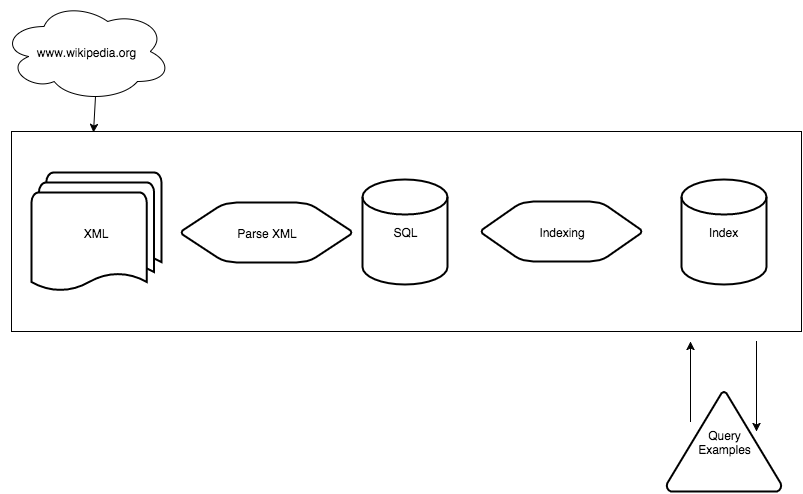
\includegraphics[width=\textwidth]{PipelineConcept}
\end{figure}


XML Parsing

\section{Database}

\section{Analysis of examples}
strucutre/characteristics of an example\\
what is good and bad example

\cleardoublepage